\documentclass[sigconf]{acmart}

\usepackage{graphicx}
\usepackage{booktabs} % For formal tables

\title{Flappy Bird with NEAT: A Neuroevolution-Based Gameplay Agent}

\author{Brady Scaggari}
\begin{document}

\maketitle

\section{Motivation}
The motivation behind this project arises from a broader interest in how neuroevolution—specifically the NEAT (NeuroEvolution of Augmenting Topologies) algorithm—can enable agents to develop complex behaviors with little to no manual feature engineering or domain-specific tuning. NEAT stands out by evolving both the topology and weights of neural networks, providing a powerful mechanism for automated learning.

Flappy Bird, a deceptively simple game, serves as an ideal testbed for this exploration due to its fast-paced, timing-sensitive dynamics and easily measurable success criteria. The visual nature of the game also allows for intuitive analysis of agent behavior, making it a practical choice for observing the learning process and evaluating the outcomes of evolution-based training. By applying NEAT in this setting, we aim to understand how well evolutionary algorithms adapt to reactive environments and how minimal input features can still result in emergent, intelligent behavior.

\section{Problem Definition}
The task involves training a neural network agent to play Flappy Bird, a side-scrolling game where the player controls a bird that must pass through gaps between vertically aligned pipes without crashing into them. The game is continuous and physics-driven, requiring precise, real-time decision-making based on limited game state information.

Our neural network receives three input features: the bird's vertical position, the vertical distance to the next pipe gap, and the horizontal distance to the next pipe. The output of the network is a decision on whether the bird should "flap" to ascend or do nothing and descend due to gravity. The core problem is not just making the bird survive longer, but doing so consistently across generations, without the network becoming overfitted to specific pipe placements or overly reliant on rigid, deterministic behaviors.

The project also seeks to examine:
\begin{itemize}
  \item How different NEAT configurations affect learning stability and generalization
  \item Whether evolved topologies demonstrate increasing complexity over time
  \item How to balance network performance with evolutionary pressure to avoid overfitting in an artificial environment
\end{itemize}

\section{Solution Explanation}

Our solution utilizes the NEAT (NeuroEvolution of Augmenting Topologies) algorithm to evolve a neural network that learns to play the Flappy Bird game effectively. The configuration parameters were carefully tuned to balance exploration, exploitation, and network complexity during evolution. This section details the architectural choices and evolutionary dynamics set by the configuration file.

\subsection{Neural Network Architecture}
The neural network begins with a minimal topology consisting of:
\begin{itemize}
  \item \textbf{3 input nodes}, representing the bird's y-position, the vertical distance to the center of the next pipe, and the horizontal distance to the next pipe.
  \item \textbf{1 output node}, which decides whether the bird should flap (output $>$ 0.5).
  \item \textbf{1 hidden node} is initialized, allowing the network to begin learning non-linear representations from the start.
\end{itemize}
The network is \textbf{feedforward} by default (\texttt{feed\_forward = True}) and starts with \texttt{full\_direct} connections between inputs and outputs.

Figure~\ref{fig:neat-neat} illustrates the evolved topology of the winner after only one generation.

\begin{figure}[H]
  \centering
  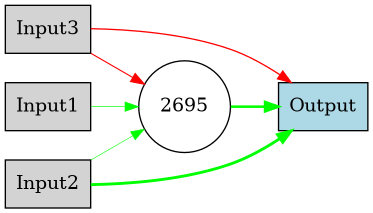
\includegraphics[width=0.85\linewidth]{best_network.png}
  \caption{Visualization of a NEAT-evolved neural network for Flappy Bird}
  \label{fig:neat-neat}
\end{figure}

This diagram represents the genome of an agent that successfully learned to play Flappy Bird using three input features:
\begin{itemize}
  \item \textbf{Input 0}: Bird's vertical position
  \item \textbf{Input 1}: Horizontal distance to the next pipe
  \item \textbf{Input 2}: Vertical distance to the center of the next pipe gap
\end{itemize}

The inputs feed into a hidden node (\textbf{Hidden 70}) as well as directly into the output node (\textbf{0}). This shows off NEAT's flexibility in forming topologies over time.

There are also constant \textbf{bias nodes} (labeled as -1, -2, -3) connected to both the hidden and output nodes. These biases help shift activation thresholds, ultimately
improving decision making and learning stability.

The output node determines whether the bird should flap or not, based on a simple rule:
\begin{itemize}
  \item If the output $>$ 0.5 $\Rightarrow$ Flap
  \item If the output $\leq$ 0.5 $\Rightarrow$ Do nothing
\end{itemize}

Over generations, NEAT evolves such topologies by adding nodes and connections through mutation, shaping more expressive and capable decision policies with minimal human intervention.

\subsection{Activation and Mutation Functions}
To promote non-linear decision-making, NEAT selects from a set of activation functions with a mutation probability:
\begin{itemize}
  \item \texttt{activation\_options = tanh, sigmoid}
  \item \texttt{activation\_mutate\_rate = 0.1}
\end{itemize}
Initially, the \texttt{tanh} function is favored, providing a smooth, bounded range from -1 to 1.

\subsection{Connection and Node Mutations}
Network complexity evolves dynamically:
\begin{itemize}
  \item \textbf{Connection addition/removal}: With probabilities of 0.3 each, new links can form between neurons while redundant ones are pruned.
  \item \textbf{Node addition/removal}: Occurs with a probability of 0.2, allowing for topological innovation over generations.
  \item \textbf{Weight mutation}: Set to 0.8, encouraging aggressive search through different weight values. Mutations follow a normal distribution with a mean of 0 and a standard deviation of 2.
\end{itemize}

\subsection{Bias and Response Mutation}
The network’s nodes can adapt their responsiveness and biases:
\begin{itemize}
  \item \textbf{Bias mutation}: Enabled with a high rate (0.3), enabling flexible thresholds for node activation.
  \item \textbf{Response mutation}: Disabled in this setup to avoid complicating learning with fluctuating sensitivity.
\end{itemize}

\subsection{Speciation and Stagnation Control}
NEAT includes speciation to preserve innovation and avoid premature convergence:
\begin{itemize}
  \item \texttt{compatibility\_threshold = 3.0} maintains diverse species.
  \item Each species is tracked by its maximum fitness, with \texttt{max\_stagnation = 20}, after which unproductive species are removed.
\end{itemize}

\subsection{Reproduction and Selection Pressure}
To ensure a mix of exploitation and innovation:
\begin{itemize}
  \item \textbf{Elitism}: The top 2 individuals per generation are carried forward (\texttt{elitism = 2}).
  \item \textbf{Survival threshold}: Only the top 20\% of individuals in each species are allowed to reproduce.
  \item \textbf{Minimum species size}: Set to 2, avoiding degenerate species.
\end{itemize}

\subsection{Fitness and Population}
The population is fixed at \texttt{pop\_size = 100}, and fitness is evaluated using a maximum criterion:
\begin{itemize}
  \item The goal is to reach \texttt{fitness\_threshold = 500}, representing a high-performance agent that can survive long runs through the game.
  \item If extinction occurs, \texttt{reset\_on\_extinction = False} ensures that evolution halts, highlighting the need for sustainable diversity.
\end{itemize}

This configuration enables a gradual and robust evolution of gameplay intelligence without manual tuning of the network structure. As generations proceed, the system adapts the complexity and decision-making precision of agents, aiming to discover networks that generalize well across varying pipe positions and speeds.


\section{Data Description}
NOT DONE

\section{Result Analysis}
PLEASE DO THIS THESE ARE SOME THINGS I THINK THAT WOULD BE IMPORTANT TO GO OVER
\begin{itemize}
  \item Learning curve of agent performance over generations
  \item Standard deviation of fitness scores
  \item Discussion of network topology changes
\end{itemize}

\section{Conclusion}
This project demonstrates the feasibility of using NEAT for real-time gameplay agents. Our modular setup supports future enhancements including visualization, reward shaping, and experimentation with different activation functions.

\end{document}